\def\baselinestretch{1}
\chapter{GPU (Graphics Processing Unit)} \label{cap:GPU}
\def\baselinestretch{1.66}

\section{Cosa sono le GPU}
\noindent Con il termine \textit{\textbf{GPU (Graphics Processing Unit)}} si intendono dei microprocessori \footnote{Tipologia particolare di processore; più precisamente è un circuito elettronico dedicato all'elaborazione di istruzioni di dimensioni molto ridotte} nati per essere adoperati principalmente nel campo della \textit{\textbf{computer grafica}} \footnote{Insieme di tecniche e algoritmi informatici per la generazione e la modifica di immagini e video digitali.}: rendering e operazioni grafiche pricipalmente. Grazie alla loro capacità di eseguire calcoli in parallelo, ben presto furono utilizzate anche in applicazioni di tipo \textit{\textbf{general purpose}}, ossia applicazioni che non coinvolgessero eslusivamente solo il campo della computer grafica. In particolar modo, data la loro elevata capacità computazionale, le GPU si prestano molto bene in ambito scientifico, dove sono utilizzate per risolvere problemi particolarmente complessi che richiederebbero tempi considerevolmente lunghi per essere risolti dai normali processori.

\section{Architettura GPU vs architettura CPU}
\noindent Le \textit{\textbf{GPU (Graphics Processing Unit)}} sono specializzata per il calcolo ad alta intensità e altamente parallelo - esattamente ciò che riguarda il rendering grafico - e quindi progettata in modo tale che più transistor siano dedicati all'elaborazione dei dati piuttosto che alla memorizzazione nella cache di quest'ultimi e al controllo del flusso, come accade ad esempio nelle \textit{\textbf{CPU (Central Processing Unit)}} \footnote{Componente di un calcolatore (detta anche processore) che carica le istruzioni dei programmi in memoria, le interpreta e manipola i dati di conseguenza.}, rendendo difatti più veloci ed efficienti le GPU rispetto alle CPU.
\begin{figure}[ht!]
    \centering
    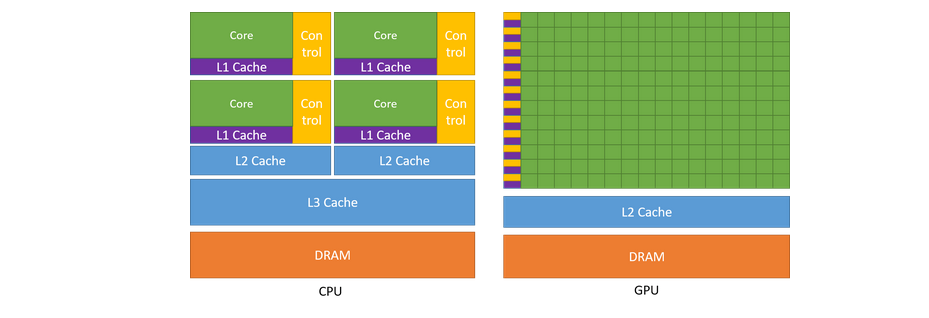
\includegraphics[scale=0.6]{img/CPUvsGPU.png}
    \caption{Architettura CPU vs architettura GPU}
\end{figure}
\noindent Questa differenza di capacità tra la GPU e la CPU esiste perché sono progettate con obiettivi diversi in mente. Mentre la CPU è progettata per eccellere nell'eseguire una sequenza di operazioni, chiamate \textit{\textbf{thread}}, il più velocemente possibile e può eseguire alcune decine di questi thread in parallelo, la GPU è progettata per eccellere nell'eseguirne migliaia in parallelo.
\noindent In generale, un'applicazione ha un mix di parti parallele e parti sequenziali, quindi i sistemi sono progettati con un mix di GPU e CPU per massimizzare le prestazioni complessive. Le applicazioni con un elevato grado di parallelismo possono sfruttare la natura massicciamente parallela della GPU per ottenere prestazioni più elevate rispetto alla CPU\cite{Nvidia-architecture}.

\section{Il ruolo di NVIDIA}
\noindent Nel 1999 NVIDIA inventa l'unità di elaborazione grafica o \textit{\textbf{GPU (Graphics Processing Unit)}}, un'idea che rivoluzionerà l'intero settore. Il lancio di GeForce 256 la descrive come prima GPU del mondo, coniando un termine che NVIDIA definisce come \emph{"un processore a chip singolo con motori integrati di trasformazione, illuminazione, creazione/clipping di triangoli e rendering in grado di elaborare un minimo di 10 milioni di poligoni al secondo"}. Le attuali GPU elaborano oltre 7 miliardi di poligoni al secondo\cite{Nvidia-story}. 
Nel corso degli anni, NVIDIA si è affermata come azienda leader nel settore, sviluppando architetture per le GPU via via più complesse e performanti. Oggi NVIDIA opera principalmente nel campo della \textit{\textbf{computer vision}} \footnote{Un campo dell'intelligenza artificiale (IA) che permette ai computer e ai sistemi di ricavare informazioni significative da immagini digitali, video e altri input visivi - e intraprendere azioni o formulare delle segnalazioni sulla base di tali informazioni.}, come ad esempio l'addestramento di veicoli per la guida autonoma.

\section{Nvidia CUDA (Compute Unified Device Architecture)}
\noindent Nel 2006 NVIDIA crea \textit{\textbf{CUDA (Compute Unified Device Architecture)}}\cite{Nvidia-story}, un'architettura sviluppata con lo scopo di utilizzare le proprie GPU dalla serie GeForce 8 in poi per eseguire eaborazioni che non siano quelle tradizionalmente legate all'ambito della computer grafica.
In questo modo, le GPU diventano totalmente programmabili e viene aggiunto il supporto a linguaggi di programmazione ad alto livello come ad esempio C e C++. Grazie all'ambiente di sviluppo CUDA è possibile utilizzare specifiche API per programmare le GPU. Ovviamente, ci sono delle specifiche API per ogni linguaggio supportato da CUDA.
\begin{figure}[h!]
    \centering
    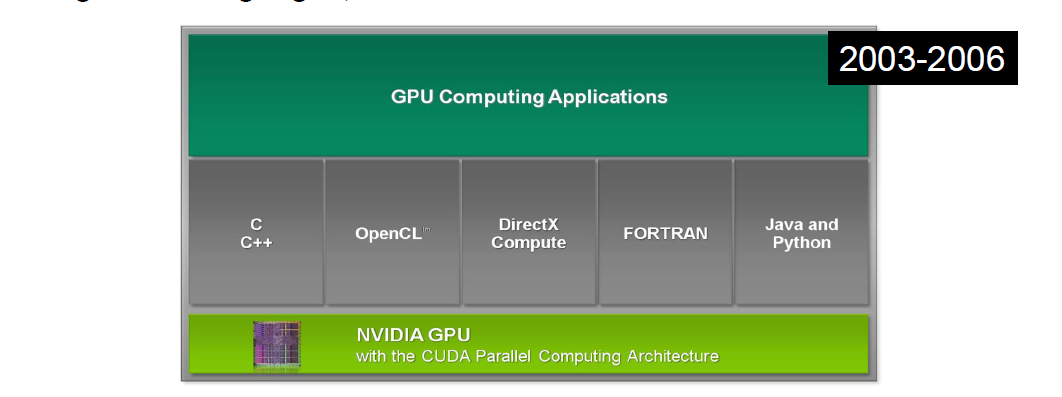
\includegraphics[scale=0.6]{img/cuda_supported_programming_languages.png}
    \caption{Alcuni dei linguaggi supportati dall'ambiente di sviluppo CUDA.}
\end{figure}

\subsection{Modello di programmazione CUDA}
\noindent Il modello di programmazione CUDA considera CPU e GPU come due macchine distinte, denominate \textit{\textbf{host}} e \textit{\textbf{device}}. Un'applicazione CUDA combina parti sequenziali (eseguite dall'host) e parti parallele (eseguite dal device). La parte di codice che lavora in parallelo è chiamata \textit{\textbf{kernel}}. L'host invoca i kernel configurando il device per l'esecuzione in parallelo, passandogli alcuni parametri. Il device può eseguire solo un kernel alla volta.

\subsubsection{Thread, block e grid}
\noindent L'unità base del parallelismo in CUDA è chiamata \textit{\textbf{thread}}: più thread eseguiti sul device eseguono lo stesso flusso di istruzioni su dati differenti, creando quello che NVIDIA ha ribattezzato come paradigma \textit{\textbf{SIMT (Single Instruction Multiple Threads}}, simile al paradigma \textit{\textbf{SIMD (Single Instruction Multiple Data)}} della \textit{\textbf{tassonomia di Flynn}}\footnote{La tassonomia di Flynn è un sistema di classificazione delle architetture dei calcolatori che classifica i sistemi di calcolo a seconda della molteplicità del flusso di istruzioni e del flusso dei dati che possono gestire}.
I thread sono raggruppati in blocchi (\textit{\textbf{blocks}}), questi blocchi vengono eseguiti sullo stesso \textit{\textbf{Streaming Multiprocessor (SM)}} e condividono una memoria condivisa che d'ora in avanti chiameremo \textit{\textbf{shared memory}}.
I blocchi sono raggruppati in una griglia (\textit{\textbf{grid}}), tutti i blocchi del device condividono una \textit{\textbf{global memory}} (la memoria della GPU). Nella Figura \ref{fig:kernel_configuration} possiamo osservare una possibile configurazione di thread e blocchi in una griglia.
\begin{figure}[h!]
    \centering
    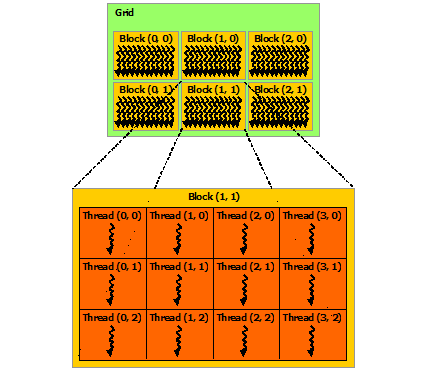
\includegraphics[scale=0.5]{img/threads_blocks_grid.png}
    \caption{Una possibile configurazione di un kernel CUDA. Una griglia 2D con $2 \times 3$ blocchi con $3 \times 4$ thread per ogni blocco.}
    \label{fig:kernel_configuration}
\end{figure}

\subsubsection{Struttura base di un'applicazione CUDA}
\noindent La struttura base di un'applicazione può essere riassunta nel seguente modo:
\begin{itemize}
    \item Prima di chiamare il kernel, l'host trasferisce i dati da elaborare sulla GPU;
    \item L'host chiama il kernel, passandogli gli argomenti appropiati di modo da permetterne la sua esecuzione;
    \item Dopo che i dati sono stati elaborati, vengono riportati sull'host dalla memoria del device.
\end{itemize}
\begin{figure}[h!]
    \centering
    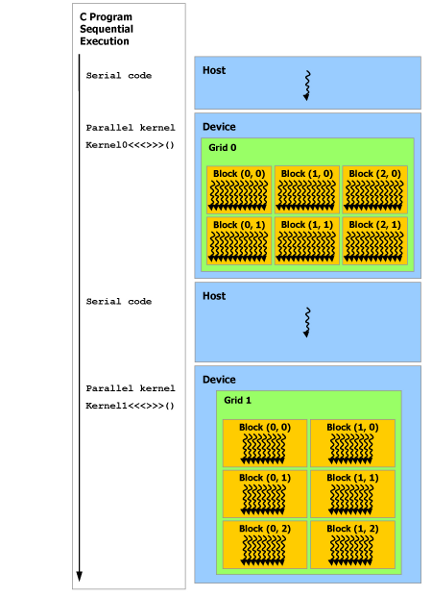
\includegraphics[scale=0.56]{img/heterogeneous-programming.png}
    \caption{Struttura base di un'applicazione cuda che evidenzia le parti sequenziali e quelle parallele.}
    \label{fig:hetero_programming}
\end{figure}

\subsection{Organizzazione della memoria}
\noindent La memoria del dispositivo è suddivisa in diverse tipologie distinguibili dalla latenza nel tempo di accesso e da quale unità è accessibile:
\begin{itemize}
    \item \textit{\textbf{Constant memory}}: area di sola lettura, per la lettura accelerata da parte di tutti i thread.
    \item \textit{\textbf{Texture memory}}: area di sola lettura, ottimizzata per la lettura e accessibile da tutti i thread.
    \item \textit{\textbf{Global memory}}: area di lettura/scrittura, esterna ai multiprocessori e condivisa tra i thread. In questo spazio, controllato dall'host, si trovano le variabili trasferite dall'host al dispositivo e viceversa. Il tempo di accesso a questa memoria è molto elevato, ma poiché essa costituisce l'interfaccia immediata con la memoria RAM della CPU, i dati devono passare per forza dalla global memory.
\end{itemize}
\begin{figure}[h!]
    \centering
    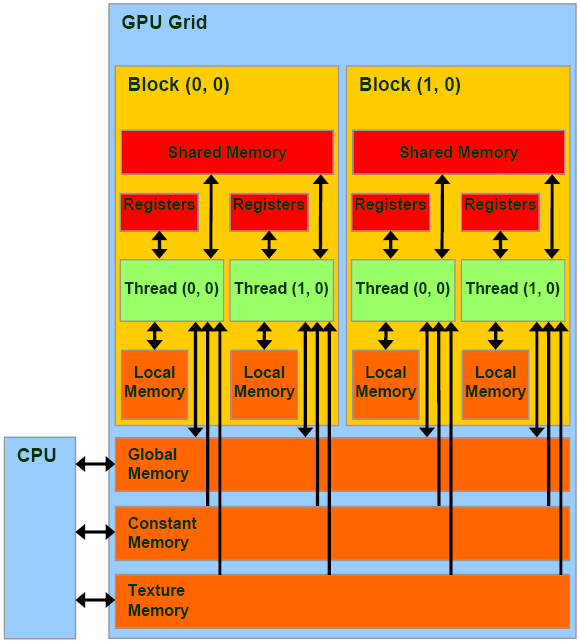
\includegraphics[scale=0.4]{img/CUDA-memory-model.png}
    \caption{Organizzazione della memoria nell'architettura CUDA.}
    \label{fig:cuda_memory_model}
\end{figure}

\subsection{Shared memory e coalescenza}
\noindent Alla classificazione della memoria della sezione precedente che si concentra sulle memorie esterne ai blocchi, possiamo aggiungere un'altra classificazione, quella delle memorie che troviamo all'interno di ciascun blocco (come riferimento si tenga presente la Figura \ref{fig:cuda_memory_model}):
\begin{itemize}
    \item \textit{\textbf{Register memory}}: memoria a bassa latenza \footnote{La latenza rappresenta i cicli di clock della memoria necessari a reperire un dato in essa memorizzato. }, privata per ogni singolo processore e accessibile da un solo thread.
    \item \textit{\textbf{Local memory}}: spazio privato per ogni singolo thread in cui sono memorizzate le variabili locali.
    \item \textit{\textbf{Shared memory}}: area di accesso a bassa latenza condivisa tra tutti i thread dello stesso blocco.
\end{itemize}
\noindent La chiave per ottenere prestazioni soddisfacenti è minimizzare gli accessi alla global memory sfruttando il più possibile la shared memory. La memoria condivisa può essere utilizzata sia come spazio privato che come spazio condiviso per la comunicazione tra i thread dello stesso blocco. Sfruttando questa capacità, i thread di uno stesso blocco possono collaborare per caricare dalla global memory alla shared memory i dati che devono essere elaborati. Successivamente provvederanno ad elaborare i dati sfruttando la minor latenza offerta dalla shared memory. Dunque i passi che ciascun thread deve eseguire sono:
\begin{itemize}
    \item caricare i dati dalla global memory alla shared memory;
    \item sincronizzare i thread di un blocco
    \item elaborare i dati nella shared memory
    \item sincronizzare nuovamente i thread per assicurarsi che tutti i thread abbiano eseguito i calcoli
    \item trasferire i dati dalla shared alla global memory
\end{itemize}
Per ottenere accessi alla memoria più veloci, i 16 KB destinati alla shared memory e condivisi tra tutti gli streaming multiprocessor, sono divisi in 16 banchi ciascuno da 1 KB, uno per ogni processore.
Come è facile intuire, per sfruttare questa memoria sono necessarie modifiche sostanziali al codice e una completa riprogettazione degli algoritmi. Tuttavia il lavoro viene ripagato da performance nettamente migliori rispetto all'algoritmo che non fa uso della shared memory. \\
I trasferimenti di dati da e verso la memoria sono governati dalla \textit{\textbf{coalescenza}}. Si indica con questo termine una serie di restrizioni che consentono di unire più accessi alla memoria in un'unica transazione. Gli accessi al kernel sono chiamati coalescenti se i thread con identificatori\footnote{Ogni CUDA thread ha un proprio identificatore (id) che lo identifica nel blocco.} consecutivi accedono a posizioni di memoria contigue utilizzando la stessa istruzione. Ciò deriva da una speciale configurazione di thread che possono essere raggruppati in \textit{\textbf{warp}}, gruppi di 32 thread che eseguono tutti la stessa istruzione.
\begin{figure}[h!]
    \centering
    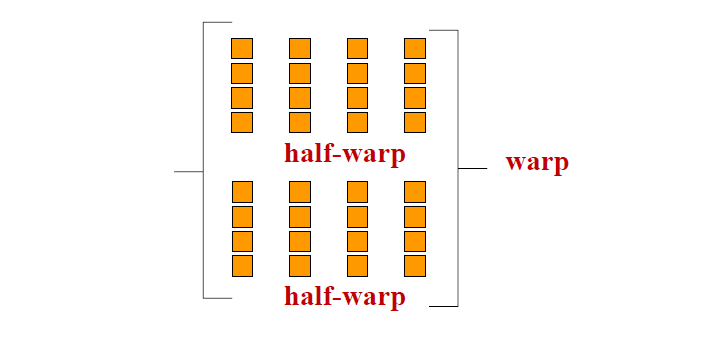
\includegraphics[scale=0.8]{img/cuda_warp.png}
    \caption{Un warp di thread (32 thread) diviso un due warp da 16 thread ciascuno.}
    \label{fig:cuda_warp}
\end{figure}

\section{API di CUDA per il linguaggio C}
\noindent CUDA mette a disposizione delle API per il linguaggio C, che rendono semplice e intuitivo l'allocazione di dati sul device, il trasferimento di dati da host a device e viceversa, la creazione e la configurazione di kernel e molto altro. Nelle sezioni successive verrà analizzata la struttura base di programma CUDA, concentrandosi in particolar modo su quali sono le funzioni di libreria che vengono più spesso utilizzate e come i dati devono essere allocati. Inoltre viene proposto un esempio banale di kernel che effettua la somma puntuale di due vettori di interi.

\subsection{Struttura base di un programma CUDA}
\noindent Un programma in \textit{\textbf{CUDA C}} deve necessariamente includere l'header \texttt{<cuda.h>}, ove sono contenute tutte le funzioni di libreria necessarie al programma. La struttura base di un programma può essere riassunta nei seguenti passi:
\begin{itemize}
    \item dichiarazione delle variabili dell'host
    \item dichiarazione delle variabili del device
    \item allocazione dei dati dell'host con \texttt{malloc}
    \item allocazione dei dati del device con \texttt{cudaMalloc}
    \item inizializzazione dei dati dell'host
    \item copia dei dati da host a device con la funzione \texttt{cudaMemcpy}
    \item invocazione kernel: configurazione dei parametri
    \item copia dei risultati da device a host con la funzione \texttt{cudaMemcpy}
    \item deallocazione dei dati dell'host con la funzione \texttt{freee}
    \item deallocazione dei dati del device con la funzione \texttt{cudaFree}
\end{itemize}
Tutte le operazioni in CUDA sono fatte per mezzo di puntatori. Vettori e matrici devono essere allocati dinamicamente e in particolare, le matrici devono essere allocate come se fossero dei vettori. Esempio: se la matrice $A$ ha dimensioni $M \times N$, deve essere allocato un array di dimensioni $M \times N$.

\lstinputlisting[language=C, caption=Esempio allocazione matrice dell'host con CUDA]{code/cuda_allocation.c}

\noindent Di conseguenza, per accedere ad un elemento della matrice \texttt{a} non si usa la seguente sintassi \texttt{a[i][j]} ma la sintassi per accedere ad un elemento in posizione \texttt{i,j} è \texttt{a[i * N + j]}, dove $N$ è il numero di colonne della matrice è costituisce la cosiddetta \textit{\textbf{leading dimension}}\footnote{La leading dimension per una matrice è un incremento utilizzato per trovare il punto iniziale per gli elementi della matrice in ogni colonna successiva della matrice.\cite{leading-dimension}}. \\
\noindent Di seguito si riporta un banale programma cuda che non fa altro che copiare un array da host a device e poi di nuovo da device ad host.
\vspace{0.5cm}

\noindent Librerie da includere:
\lstinputlisting[language=C, firstline=1, lastline=3, caption=Librerie richieste dall'ambiente CUDA]{code/first_cuda.c}

\newpage
\noindent Funzione main del programma:
\lstinputlisting[language=C, firstline=9, lastline=62, caption=Inizializzazione e copia di una matrice host-device e device-host]{code/first_cuda.c}

\noindent Funzioni helper:
\lstinputlisting[language=C, firstline=64, lastline=85, caption=Funzioni utilizzate nel precedente listato]{code/first_cuda.c}

\subsection{Funzioni di libreria più utilizzate}
\noindent Dopo aver illustrato un semplice esempio di programma CUDA C, analizziamo un po' più nel dettaglio quali sono le funzioni di libreria più utilizzate.

\subsubsection{Allocazione della memoria su GPU}
\begin{lstlisting}[language=C]
    cudaError_t cudaMalloc(void **devPtr, size_t size);
\end{lstlisting}
\begin{itemize}
    \item \texttt{devPtr} - puntatore all'area di memoria da allocare sul device
    \item \texttt{size} - la dimensione in byte dell'area da allocare
\end{itemize}

\subsubsection{Deallocazione della memoria su GPU}
\begin{lstlisting}[language=C]
    cudaError_t cudaFree(void *devPtr);
\end{lstlisting}
\begin{itemize}
    \item \texttt{devPtr} - puntatore all'area di memoria da deallocare sul device
\end{itemize}

\subsubsection{Scambio di dati tra CPU e GPU}
\begin{lstlisting}[language=C]
    cudaError_t cudaMemcpy(
        void *dest, 
        void *src, 
        size_t nBytes, 
        enum cudaMemcpyKind
    );
\end{lstlisting}
\begin{itemize}
    \item \texttt{dest} - puntatore all'area di memoria in cui copiare
    \item \texttt{src} - puntatore all'area di memoria da cui copiare
    \item \texttt{nBytes} - la dimensione in byte dell'area di memoria da copiare
    \item \texttt{cudaMemcpyKind} - indica la direzione della copia. È una variabile che può assumere i seguenti valori:
    \begin{itemize}
        \item \texttt{cudaMemcpyHostToHost} copia i dati da host a host
        \item \texttt{cudaMemcpyHostToDevice} copia i dati da host a device
        \item \texttt{cudaMemcpyDeviceToHost} copia i dati da device a host
        \item \texttt{cudaMemcpyDeviceToDevice} copia i dati da device a device
    \end{itemize}
\end{itemize}

\subsection{Creazione e configurazione di un kernel}
\noindent Di seguito si riporta l'esempio di un kernel che effettua la somma puntuale di due vettori di \texttt{float} e la memorizza in un terzo vettore. Per semplicità si omettono tutte le parti relative all'allocazione e alla deallocazione di variabili.

\vspace{0.5cm}
\lstinputlisting[language=C,  caption=Configurazione di un kernel per la somma di due vettori.]{code/kernel_example.c} \label{list: ex01}
\vspace{0.5cm}

\noindent Le funzioni CUDA hanno lo stesso prototipo delle solite funzioni C precedute da uno di questi qualificatori:
\begin{itemize}
    \item \texttt{\_\_global\_\_} : per le funzioni chiamate dall'host ed eseguite sul device (i kernel)
    \item \texttt{\_\_device\_\_} : per le funzioni chiamate dal device ed eseguite sul device
    \item \texttt{\_\_host\_\_}: (opzionale) per le funzioni eseguite dalla CPU
\end{itemize}

\noindent Il tipo di dato \texttt{dim3} è un tipo predefinito di CUDA che rappresenta un vettore di tre interi; questi tre campi sono accessibili con le notazioni \texttt{.x}, \texttt{.y}, \texttt{.z} e servono per indicare il numero dei fili o il numero dei blocchi in una particolare direzione; gli eventuali campi non dichiarati vengono automaticamente impostati a 1.
\begin{itemize}
    \item \texttt{nBlocks} è il numero di blocchi della griglia, può essere 1D o 2D
    \item \texttt{nThreadsPerBlock} è il numero di thread per un singolo blocco (1D, 2D o 3D)
\end{itemize}

\subsubsection{Esempio}
\noindent Supponiamo di usare $N = 12$. Fissando il numero di blocchi a 3 come nell'esempio \ref{list: ex01}, il numero di thread per ciascun blocco sarà pari a 4, poiché $12 / 3 = 4$. Nel caso N non fosse stato esattamente divisibile per il numero di blocchi, al numero di thread sarebbe stato aggiunto un 1 e alcuni thread non avrebbero partecipato al calcolo della somma.

\begin{figure}[h!]
    \centering
    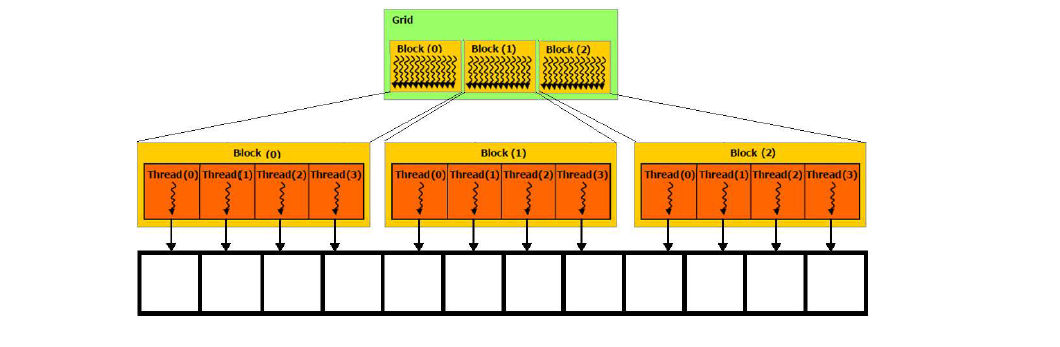
\includegraphics[scale=0.6]{img/kconf.png}
    \caption{Configurazione del kernel CUDA \texttt{VecAdd} con N = 12 e numero di blocchi pari a 3.}
\end{figure}